\section{Motivation}
\label{sec:motivation}


% \begin{table*}[]
% \begin{tabular}{|l|l|l|}
% \hline
%                                          & \textbf{ESCHER}                          & \textbf{Omega}                                   \\ \hline
% \textbf{Scheduler implementation by}     & Framework (constraints specified by application) & Application                                      \\ \hline
% \textbf{Best suited for}                      & Short lived tasks                        & Long running tasks (fewer OCC conflicts)          \\ \hline
% \textbf{Concurrency model}               & Resource ownership granted by parent ESL & Optimistic concurrency control with shared state \\ \hline
% \textbf{Cluster-wide policy enforcement} & Managed by parent ESL                    & Free-for-all, hard to enforce cluster policies   \\ \hline
% \textbf{Conflict resolution} & Done by framework                    & Done by application   \\ \hline
% \end{tabular}
% \caption{ESCHER vs Omega}

% \end{table*}

%\name{} is motivated by the need of many modern distributed applications for fine-grained scheduling control.
\Cref{tab:sched-pols} lists some common scheduling policies required by modern distributed applications and their off-the-shelf support across different frameworks and specialized schedulers. 
None of the schedulers support all policies, and many were built as a one-off solution to achieve a composition of these policies. 
New applications which require a new policy must find alternate methods of executing it - either by using some mechanism provided by the scheduler, such as labels, or writing their own scheduler from scratch. %\romil{Move the labels to after distributed training?}
We now give a motivating example that is insufficiently served by existing schedulers and describe how \name{} fills this gap.
%As a result, researchers and practitioners have developed specialized frameworks to support these workloads. Unfortunately, building such one-off solutions is expensive and does not scale. 

% https://docs.google.com/spreadsheets/d/16M7Ia2e4X7hofFKPAhwRx6LiYlhBFzlqwzldHgewwCQ/edit?usp=sharing
%\newcommand{\centered}[1]{\begin{tabular}{l} #1 \end{tabular}}
\newcommand\colw{0.8}

\newcommand{\xmark}{\ding{55}}

\begin{table}[!t]
  \small
  \centering
  \begin{xtabular}{|p{0.45\linewidth}|
  p{\colw em}|p{1.6em}|p{\colw em}||p{\colw em}|p{\colw em}|p{\colw em}|}
  \cline{2-7}
  \multicolumn{1}{c|}{}  &  \multicolumn{3}{c||}{\textbf{Framework}} & \multicolumn{3}{c|}{\textbf{Scheduler}}\\
  \hline
    \textbf{Policy} 
  \vspace{13mm} & 
  \textbf{\rotatebox[origin=c]{90}{YARN CS~\cite{yarn}}} &
  \textbf{\rotatebox[origin=c]{90}{\parbox{2.2cm}{Kubernetes~\cite{kubernetes} Core / Labels}}} &
  \textbf{\rotatebox[origin=c]{90}{Spark~\cite{spark}}} &
  \textbf{\rotatebox[origin=c]{90}{Sparrow~\cite{sparrow}}} &
  \textbf{\rotatebox[origin=c]{90}{Gandiva~\cite{gandiva}}} &
  \textbf{\rotatebox[origin=c]{90}{Gorila~\cite{gorila}}}
  \\
  \hline
  
  % Begin info
  
  \textbf{Task co-location}\newline
  Place $n$ tasks on the same physical machine.
  %\vspace{1mm}
    % \begin{minted}[autogobble]{python}
    % coloc_tasks = [...]
    % res_constraint = sum([t.resources for t in coloc_tasks])
    % set_resource("coloc-group", len(coloc_tasks), res_constraint)
    % for task in coloc_tasks:
    %     task.launch(resources={"coloc-group": 1})
    % \end{minted}
  &
  $\checkmark$& % YARN CS
  $\checkmark\text{/\checkmark}$& % Kubernetes
  $\text{\xmark}$& % Spark
  $\checkmark$& % Sparrow
  $\checkmark$& % Gandiva
  $\checkmark$% Gorila
  \\
  \hline
  
  \textbf{Data locality}\newline
  Place tasks with operands.
  \vspace{0.01em}
    % \begin{minted}[autogobble]{python}
    % data_addr = nodeid  # Node id where the data is
    % set_resource("data-loc", 1, data_addr)
    % task.launch(resources={"data-loc": 1})
    % \end{minted}
  &
  $\checkmark$& % YARN CS
  $\checkmark\text{/\checkmark}$& % Kubernetes
  $\checkmark$& % Spark
  $\checkmark$& % Sparrow
  $\text{\xmark}$& % Gandiva
  $\text{\xmark}$ % Gorila
  \\
  \hline
  
%   \textbf{Static Load Balancing}\newline
%   Given $n$ tasks, evenly spread them out across $m$ workers.
%   %\vspace{1mm} 
% %     \begin{minted}[autogobble]{python}
% %   resource_capacity = ceiling(num_tasks/num_nodes)
% %   for node in nodes:
% %     set_resource("load_bal", resource_capacity, node)
% %   for task in tasks:
% %     task.launch(resources = {"load_bal": 1})
% %     \end{minted}
%   &
%   $\checkmark$& % YARN CS
%   $\checkmark\text{/\checkmark}$& % Kubernetes
%   $\checkmark$& % Spark
%   $\checkmark$& % Sparrow
%   $\checkmark$& % Gandiva
%   $\checkmark$% Gorila
%   \\
%   \hline
  
  \textbf{Elastic Load Balancing}\newline
  Given an unknown number of tasks, evenly spread them out across $m$ workers. 
  \vspace{-4mm}
%   \begin{minted}[autogobble]{python}
%     def load_monitor():
%       while True:
%         avail_res = get_cluster_status()
%         if avail_res["load_bal"] == 0 on all nodes:
%             set_resource("load_bal", increment 1, all_nodes)
%         if avail_res["load_bal"] >= 1 on all nodes:
%             set_resource("load_bal", decrement 1, all_nodes)

%     def dynamic_load_balancing():
%       load_monitor.launch()
%       for task in tasks:
%         task.resources = {"load_bal": 1}
%         task.launch()
%     \end{minted}
  &
  $\checkmark$& % YARN CS
  $\checkmark$\text{{/\xmark}}& % Kubernetes
  $\text{\xmark}$& % Spark
  $\checkmark$& % Sparrow
  $\checkmark$& % Gandiva
  $\checkmark$% Gorila
  \\
  \hline
  
  \textbf{Bin-packing}\newline 
  Given an unknown number of incoming tasks, minimize the number of workers used to complete the tasks.
  %\vspace{1mm}
  &
  $\checkmark$& % YARN CS
  $\checkmark$\text{{/\xmark}}& % Kubernetes
  $\text{\xmark}$& % Spark
  $\text{\xmark}$& % Sparrow
  $\checkmark$& % Gandiva
  $\text{\xmark}$% Gorila
  \\
  \hline
  
  \textbf{Anti-affinity}\newline 
  Given two tasks, place them on distinct nodes.
  &
  $\checkmark$& % YARN CS
  $\checkmark$\text{{/\checkmark}}& % Kubernetes
  $\text{\xmark}$& % Spark
  $\text{\xmark}$& % Sparrow
  $\checkmark$& % Gandiva
  $\text{\xmark}$% Gorila
  \\
  \hline
  
  \textbf{Gang scheduling}\newline 
  Given a set of tasks, enforce all-or-none run semantics.
  \vspace{1mm}
  &
  $\text{\xmark}$& % YARN CS
  $\text{\xmark}\text{{/\xmark}}$& % Kubernetes
  $\checkmark$& % Spark
  $\text{\xmark}$& % Sparrow
  $\text{\xmark}$& % Gandiva
  $\checkmark$% Gorila
  \\
  \hline
  
  \textbf{Weighted Fair Queuing\cite{wfq}}\newline 
  Given a set of tasks, enforce priority ordering. 
  &
  $\checkmark$& % YARN CS
  $\checkmark\text{{/\xmark}}$& % Kubernetes
  $\checkmark$& % Spark
  $\checkmark$& % Sparrow
  $\text{\xmark}$& % Gandiva
  $\text{\xmark}$% Gorila
  \\
  \hline

  \textbf{Soft-constraints}\newline  
  For a priority ordering of resource constraints, schedule a task with the highest possible resource satisfiability.
  &
  $\text{\xmark}$& % YARN CS
  $\checkmark\text{{/\xmark}}$& % Kubernetes
  $\text{\xmark}$& % Spark
  $\text{\xmark}$& % Sparrow
  $\text{\xmark}$& % Gandiva
  $\text{\xmark}$% Gorila
  \\
  \hline
  
  \end{xtabular}
  \vspace{2mm}
  \caption{\small Common scheduling policies and off-the-shelf support from existing schedulers. Kubernetes comparision includes both modes of operation, using just the core scheduling functionality and using labels. In addition to these policies, ephemeral resources allow applications to specify and compose custom policies.
  %\romil{Once format is approved, reorder columns to fit the category. Frameworks: YARN, Kubernetes, Spark}
  %\swang{Make the vertical line between "Frameworks" and "Schedulers" bold}
  }
  \label{tab:sched-pols}
\end{table}

\subsection{Existing systems are hard to evolve}
\label{sec:motivation:example}

% As model size increases, 
As applications become increasingly diverse, the cluster schedulers must evolve to support novel scheduling policies required by these applications. Consider distributed training, which has emerged as a dominant ML workload. 
Multiple training jobs are often scheduled simultaneously due to multi-tenancy and individual users submitting multiple training runs in parallel to evaluate different model architectures.
This requires several distinct scheduling policies: % \rliaw{we can say something stronger here right? it's not simply an issue of supporting, there's also a hierarchical relationship}
\begin{compactitem}
\item \emph{Anti-affinity:} Evenly spread training jobs across the cluster to ensure high throughput.
\item \emph{Affinity:} Co-locate all tasks of the same training job on the same machine to avoid unnecessary data transfers.
\item \emph{Gang scheduling:} For multi-node jobs, schedule all tasks of the job simultaneously to avoid starvation.
\item \emph{Bin packing (dynamic):} Monitor job utilization and consolidate jobs to reduce resource fragmentation. % TODO: And reduce network transfers.
\end{compactitem}

Many popular schedulers implement at least one of these policies, but it is rare for them to support all four~(\Cref{tab:sched-pols}), never mind a composition of the policies.
% Monolithic schedulers tightly couple the scheduling policy and mechanism~(\Cref{fig:scheduler-architectures}a).
There are two fundamental challenges that make it difficult or infeasible to extend monolithic schedulers~(\Cref{fig:scheduler-architectures-new}a) in this way.
We use Kubernetes~\cite{kubernetes} to illustrate these challenges. %, but we stress that the following limitations are in fact \textit{fundamental} to monolithic schedulers.
% 

First, the application must \emph{express} its policy using the API chosen by the framework scheduler.
%Each scheduler exposes a different interface for policy specification.
While some schedulers support composition, it is difficult in general to design a scheduler API that can capture all possible use cases.
For example, in Kubernetes, applications specify scheduling policies with \emph{static weights} to resolve conflicts.
This can be used to express a composition of two policies that, for instance, weights affinity over anti-affinity.
However, the complexity of composition is not linear in the number of policies.
E.g., to add bin packing and prioritize it, the application would have to ensure that the weight of bin packing is always greater than the sum of weights for affinity and anti-affinity.
% Furthermore, dynamic policies like bin packing in this case cannot be expressed using only static weights.

Second, the scheduler \emph{implementation} must extend to new policies.
This is difficult because the scheduler must ensure that each new policy interfaces correctly with all other existing policies.
% This is difficult because of the tight coupling between scheduling policy and mechanism in monolithic schedulers.
% For example, while Kubernetes supports a range of policies, including affinity and anti-affinity, this list is not exhaustive.
Adding another policy requires modifying Kubernetes itself, which takes significant time and effort. Dynamic policies are even more difficult to support if the scheduler was not initially designed for it. For instance, adding gang scheduling support in Kubernetes took months of discussions and the eventual feature was not mainlined and instead implemented in an add-on scheduler ~\cite{kubernetes-gang-scheduling, kubernetes-gang-scheduling-first-comment, kubernetes-gang-scheduling-kubebatch-pr}.
Similarly, Machine Learning pipelines involve multiple interdependent tasks (e.g., data pre-processing, training, serving) defined in a DAG. Scheduling DAGs is not natively supported in Kubernetes, leading to the emergence of specialized plugins such as Kubeflow~\cite{kubeflow}.

% For example, the ability to correct previous scheduling decisions requires an entirely separate system to evict tasks in Kubernetes~\cite{kubernetes-descheduler}.
% Furthermore, this system only handles changes in the \emph{cluster} environment and does not allow changes in the \emph{application} policy.

Due to these limitations, applications must write custom schedulers to maximize performance, as Gandiva~\cite{gandiva} did for distributed training.
% Gandiva uses feedback from the application to dynamically adjust task placement, composing affinity, anti-affinity, and dynamic bin-packing.
Unfortunately, this design requires the application to implement both the policy and the scheduler \emph{mechanism}, maintaining resource state and handlers for task and resource management, coordination, node addition and deletion, etc.~(\Cref{fig:scheduler-architectures-new}b).
This is both difficult to build and extend.
E.g., Gandiva (built on Kubernetes) supports affinity, anti-affinity, and dynamic bin-packing, but the addition of gang scheduling would greatly increase the complexity of the scheduler code.
%\alexey{can we quantify this, Romil?}
Thus, Gandiva remains limited to distributed training jobs that fit on a single multi-GPU node.

% https://docs.google.com/drawings/d/1x6561xEY_K5CEV12J6dLwa7TMJqwGX-idUDL-PlSrb0/edit
% \begin{figure}[ht]
%     \centering
%     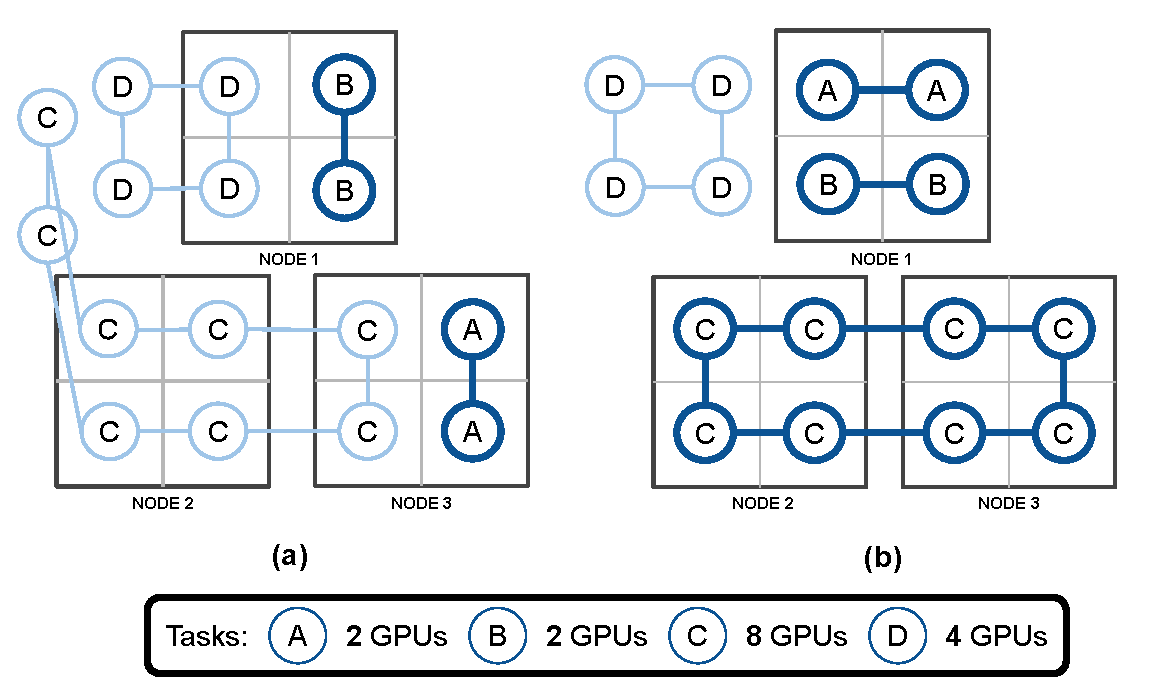
\includegraphics[width=0.95\linewidth]{escher/figures/ESCHER-training.pdf}
%     \caption{\small Task placement for 4 distributed training jobs on a cluster with 12 GPUs. Each training job comprises multiple tasks, and each task occupies 1 GPU. The jobs arrive in order from $A$-$D$, and all tasks can take a variable amount of time to start. Jobs can only make progress if all tasks are started (i.e., they require gang scheduling). \textbf{(a)} Task placement with affinity and anti-affinity, but no gang scheduling. $C$ has some tasks that are not placed before $D$ arrives, so neither $D$ nor $C$ can run. \textbf{(b)} Task placement with affinity, anti-affinity, and gang scheduling. $A$ is initially placed on Node 1 and $B$ on Node 2 (not shown). With gang scheduling, when $C$ arrives, $B$ can be migrated to Node 1 to allow $C$ to run. \romil{Candidate for cutting}}
%     \label{fig:distributed-training}
%     \vspace{-3mm}
% \end{figure}

\subsection{Static labels are insufficient}
\label{sec:motivation:label}
Some frameworks~\cite{mesos,omega,yarn,kubernetes} already support \emph{static} label creation as string key-value pairs (e.g., "v100 GPU": 1) associated with cluster nodes.
This allows cluster operators to tag nodes with physical resource attributes (e.g., CPU/GPU architecture, rack affinity) at cluster launch time, which can be requested by applications at execution time.
%Then, at execution time, an application can request task placement on nodes with specific labels, using hard or soft constraints.

% Tasks can then request placement on nodes with specific labels.
% However, in today's cluster deployments, label creation is controlled by cluster operators, not applications. This enables applications to express constraints on desired properties (e.g., CPU/GPU architecture, rack affinity, availability zone). Soft constraints are also supported, but only relative to the resource attributes.

In \name{}, we propose repurposing this API to express \emph{custom application scheduling policies}, in addition to physical resource requirements.
Unlike physical resources, which can be statically determined at a node's launch time, logical scheduling constraints may depend on run-time information.
Therefore, it is natural to extend existing static label creation APIs to \emph{ephemeral resources} that are dynamically created.

For example, to express task-task affinity between tasks $T_1$ and $T_2$, we must first learn where $T_1$ was placed before deciding the placement constraint for $T_2$.
This can be easily done through ephemeral resources: $T_1$ dynamically creates a logical resource that is required by $T_2$.
With static labels, the only option is for the application to pin $T_1$ and $T_2$ to a predetermined node.

% To express \textit{inter-task }relationships, however, requires mapping them to existing statically created resource labels. E.g., task-task affinity can only be expressed by placing task $T_1$ first and then placing task $T_2$ second with a requirement for the node label where $T_1$ landed. With ability to \textit{dynamically} create labels, applications can express inter-task constraints in a single shot, without requiring for multiple scheduling round trips necessary in TetriSched~\cite{tetrisched} and Firmament~\cite{firmament}.

For the same reason, there are some inter-task constraints that are fundamentally impossible to implement with static labels, such as scheduling policies that depend on \emph{time}.
One example is a DAG scheduling policy.
At its core, this requires a primitive that guarantees that some task $T_2$ will not run until another task $T_1$ finishes.
This is impossible to express using static labels alone, which cannot reason about the temporal ordering between two tasks.

% with cyclical/iterative behavior~\cite{naiad-sosp13}. E.g., it is impossible to express the resource schedule for two tasks $T_1$ and $T_2$ that implement an iterative computational pattern (e.g., SGD gradient calculation and model update). Dynamic ephemeral resource creation in \name{} enables $T_i$ to create a label with a logical clock suffix, incremented to reflect the iteration epoch. Each task $T_i \in \{T_1,T_2\}$ then consumes a label from the previous iteration epoch, effectively unrolling the task graph cycle~\cite{naiad-sosp13}. Capturing such dynamic behavior requires a dynamic mechanism and cannot be expressed with state-of-the-art declarative frameworks~\cite{dcm-osdi20, tetrisched}.

% provide the ability to create labels, string key-value pairs (e.g. "partition: customerA") that can be associated with nodes. These labels can subsequently be specified as necessary qualifiers for a task to be scheduled (e.g. run task $T$ only where "partition" label is "customerA"). Granting applications the ability to create and remove labels can allow applications to express custom scheduling policies. For instance, co-location can be enforced by having two tasks request a unique label in their label requirements. However, exercising scheduling control with labels has two critical shortcomings which limits its generality.

% First, node labels are static. In today's deployments, the control of label creation and deletion is primarily owned by cluster operators, who create labels when a node is added to the cluster. This limits applications to using labels created by the operators. If applications are granted the ability to create node labels, they can implement a larger set of policies, such as data-locality by creating labels where the data is generated. 

% Second, labels do not have an associated numerical capacity. Unlike a resource, tasks cannot acquire or consume labels, which makes it difficult to express policies which rely on evaluating task counts or utilization on different nodes. For instance, performing load-balancing with key-value labels would require the application to create unique labels on each node and track the number of tasks requesting each label. This is equivalent to implementing the complete scheduling logic in the application space. % Kubernetes' extended resources \cite{kubernetesextres} improves on labels by adding a numerical capacity to labels, but it remains static in it's current usage.

% \subsection{An End-to-End Argument}
% \label{sec:motivation:e2earg}

% \name{} applies the end-to-end principle~\cite{e2e-argument} to cluster scheduling by keeping the core scheduler mechanism simple yet scalable, while ephemeral resources provide applications with flexibility to express scheduling policies.
% Similar to Exokernel~\cite{exokernel}, \name{} focuses on enabling applications to implement custom scheduling policies in a heterogeneous distributed system. 
% The key design challenge is the choice of abstractions and the division of responsibilities between the system and the application.

% \name{} also follows the second core tenet of the end-to-end argument~\cite{e2e-argument}---the ability to \emph{lower} functionality into the system to enhance application performance.
% ESCHER allows the core scheduler to integrate specific policies to improve performance, as the system can itself manipulate ephemeral resources.
% For example, in \Cref{sec:eval:gangscheduling}, we show how a gang scheduling policy built on ephemeral resources can be lowered into the core scheduler.
% This maintains evolvability while enhancing performance in a layered approach.
% Framework developers can still choose which policies to support, while applications don't need to wait months for a new policy to be supported.







% The ephemeral resource API can be used to implement policies at the system level to maintain both evolvability and enhance performance in a layered approach.
% And even if the final implementation of the policy is eventually built as a separate scheduler (e.g., for performance reasons), ESCHER enables applications to use the new policy right away; the applications don't need to wait months for the new policy to be supported by the scheduler. %\romil{Move to 3.5?}
% To maintain evolvability, system-level policies must adhere to the ephemeral resources API, thus following a \emph{layered} approach.
%Still, we show that it is often possible to implement policies at the application level with sufficient performance~(\Cref{sec:eval:gangscheduling}).



% %Because modern applications require custom, composite and dynamic scheduling policies, we argue that cluster schedulers today should follow the end-to-end argument~\cite{e2e-argument}. Applications know their scheduling requirements the best and schedulers must yield policy control to them. %\romil{I think we need to justify this/claim this a bit differently}
% \name{} takes an end-to-end argument approach to cluster scheduling by implementing a simple yet flexible and scalable scheduler, while enabling applications to implement more complex scheduling policies on top.
% In particular, \name{} implements a basic resource-constrained scheduler, i.e., given a task’s resource requirements, \name{} schedules the task on a node that satisfies these requirements. For example, if a task requests 2 CPUs and 1 GPU, \name{} schedules the task on a node that has at least 2 CPUs and 1 GPU available. Besides satisfying the resources constraints, \name{} does not implement any scheduling policy. \name{} only promises that node’s resources are not overallocated; it makes no promise on which node a task is actually scheduled. Instead, it leaves to the applications to implement the scheduling policies through ephemeral resources.
% %Thus, the ESCHER scheduler design requires the framework scheduler to implement a minimalist yet flexible API, while pushing the task of specifying custom scheduling policies to the application layer~(\Cref{fig:scheduler-architectures-new}c).
% This is similar to the Exokernel~\cite{exokernel}, but the focus is on enabling the application to implement custom scheduling policies in heterogeneous distributed systems.
% % This model has several advantages:

% \romil{Bullets are candidates for cutting.}
% \begin{compactitem}
%     \item \textbf{Flexibility}. \name{} decouples application-level scheduling policies from the underlying mechanisms. This allows an application to implement a large variety of both common and custom scheduling policies.
    
%     \item \textbf{Simplicity}.
%     %To support different scheduling policies, previous solutions either end up with complex schedulers that offer a myriad of configuration knobs to the application~\cite{condor, kubernetes}, or push the complexity of implementing the scheduling policy to the application~\cite{mesos,yarn}.
%     \name{} keeps the core scheduler simple because the API that it implements is minimal.
%     Meanwhile, with the addition of modular application-level schedulers~(\Cref{sec:esl}), applications can reuse, compose, and extend common policies without complicating application-level logic.
%     %At the same time, due to their ability to express a variety of scheduling constraints (e.g., affinity, anti-affinity, gang scheduling) the interface provided to the application remains simple: just provide support for dynamically creating ephemeral resources and updating their capacities. 
%     % ESCHER creates a separation between scheduling policies and scheduling mechanisms by equipping applications to implement a variety of policies (e.g., affinity, anti-affinity, gang scheduling) with just a few lines of code (Section \ref{policies}).
    
%     \item \textbf{Performance}. Since the core scheduler API is minimal and does not incorporates application-specific logic, we can keep the scheduler design simple. This makes it much easier to scale its throughput and provide low latency.% In addition, ephemeral resources are used to specify only scheduling constraints, so they add little to no overhead on the critical path of scheduling a task.
% \end{compactitem}

% The remaining challenges are then to: 
% (1) define a common \name{} API under which frameworks can implement some common mechanism, 
% while applications can implement the policy (\Cref{sec:arch}),
% (2) generalize this API to common policies, as well as new policies not expressible in monolithic systems today (\Cref{policies}), and (3) reduce burden for those applications that require standard policies or compositions thereof, while maintaining compatibility with more complex policies ~(\Cref{sec:esl}).


% The remaining challenges are then to: 
% (1) define a common \name{} interface which frameworks can implement to provide support for a common resource matching mechanism,
% while applications can implement the policy (\Cref{sec:arch}),
% (2) use this API to implement common as well as new policies not expressible in monolithic systems today (\Cref{policies}), and 
% (3) alleviate the burden for applications that simply need standard policies or their compositions without
% giving up the generality that affords more complex policies~(\Cref{sec:esl}).

% reduce burden for those applications that require standard policies or compositions thereof, while maintaining compatibility with more complex policies ~(\Cref{sec:esl}).

% The first challenge in \name{} is then to define the core scheduler API.
% To do this, \name{} leverages a common functionality provided by cluster schedulers today: matching the application-specified resource requirements with the cluster's resource availability.
% For instance, if an application task requires two GPUs, the scheduler will schedule that task on a node that has at least two available GPUs. 

% \begin{figure}
%     \centering
%     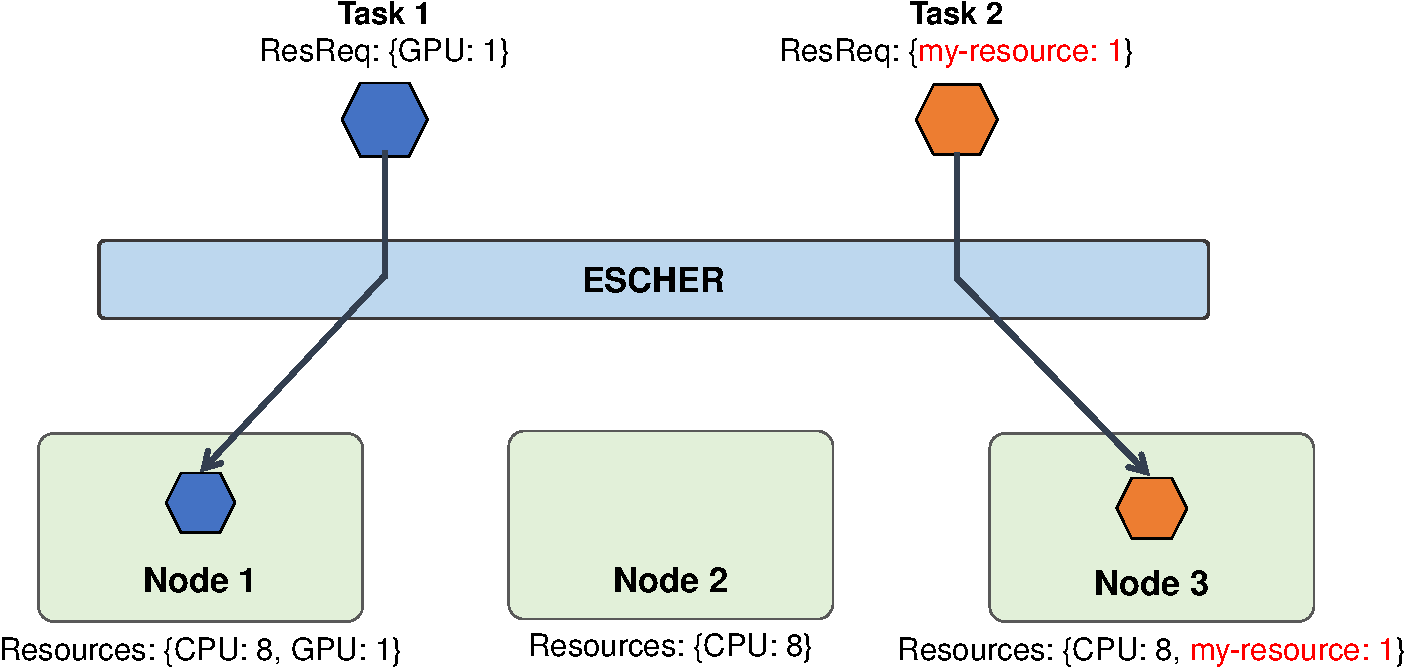
\includegraphics[width=\linewidth]{escher/figures/logicalres_demo.pdf}
%     \caption{An example demonstrating the use of ephemeral resources for targeted task placement. Applications can create custom resources, such as \emph{my-resource}, on the nodes where they wish to place a task, and then launch a task requesting \emph{my-resource} to ensure the task is placed on the desired node.}
%     %  Assuming a minimalist framework scheduler that matches task resource requests to node resource availabilities,
%     \label{fig:er-example}
% \end{figure}


% The key idea behind \name{} is then to leverage this scheduler functionality for a new type of resource: an \emph{ephemeral resource}. An ephemeral resource is a logical (i.e., non-physical) resource attribute that the application can dynamically associate with a node. The scheduler treats an ephemeral resource like any other physical resource, and aims to satisfy its capacity constraints. By associating an ephemeral resource with a particular physical node, the application can make targeted  placement decisions. As illustrated in Figure~\ref{fig:er-example}, creating a resource \lstinline{my-resource} on a node and then submitting a task requiring the resource \lstinline{my-resource} would result in the scheduler placing the task on 
% the node with enough capacity for \lstinline{my-resource}, assuming all other resource requirements are satisfied.
% Ephemeral resources follow the end-to-end argument, separating scheduling into two components: the application implements the policy, while the scheduler implements resource management.\swang{do we need this sentence? in general, a lot of this paragraph feels repetitive}
% % Surprisingly, many popular scheduling policies can be expressed in just a few lines of code using this simple mechanism, as demonstrated in Section \ref{policies}. 

% The remaining challenges in using ephemeral resources are then to: (1) generalize ephemeral resources to common policies, as well as new policies not expressible in monolithic systems today (\Cref{policies}), and (2) reduce burden for those applications that require standard policies or compositions thereof, while maintaining compatibility with more complex policies with fine-grained, dynamic scheduling decisions~(\Cref{sec:esl}).

% Why do this
% Using ephemeral resources to express scheduling constraints has several advantages. 




% Implementing the above policy is challenging because of two reasons. First, affinity and anti-affinity are conflicting requirements and therefore require an explicit specification of conflict resolution policies. Second, while the above policy can be naturally expressed as an hierarchical composition of simple policies (e.g., load-balance jobs across nodes, and co-locate all tasks of a job on the same node), very few cluster schedulers\cite{kubernetes} support such a composition. Worse, this support has limited flexibility and is restricted to a fixed set of policies. For instance, Kubernetes provides a scoring mechanism to assign weights between 13 policies, including affinity and anti-affinity policies. Moreover, these 13 policies do not constitute an exhaustive set of policies required by applications, such as gang scheduling.  %However, these policies cannot be modified by applications and custom policies cannot be integrated in the scoring computation without modifying the Kubernetes core. 
%there is no easy way to express this policy in existing cluster schedulers - they lack the primitives to adequately describe the policy. % For instance, Kubernetes \cite{kubernetes} provides a scoring mechanism to assign weights between affinity and anti-affinity policies, but does not allow a dynamic adjustment of  % \rliaw{the fundamental limitation of policy expression is not clear from the intro.}. 

% As a result, a new specialized scheduler, Gandiva~\cite{gandiva}, has been recently proposed to implement this policy. In addition to providing support for affinity and anti-affinity, Gandiva also implements job migration to help with resource de-fragmentation, i.e., consolidate small jobs on a subset of nodes to leave full nodes available to larger jobs.

% Not only sharing a cluster across multiple training jobs requires building a new scheduler, such as Gandiva, but once built, such a scheduler is not easy to extend. Currently, Gandiva is limited to distributed training jobs that fit on a single multi-GPU node. Thus, one natural extension is supporting distributed training on multiple nodes through gang scheduling. However, this is fundamentally challenging as the existing scheduler already maintains multiple state variables and checks for affinity, anti-affinity and job migration. Adding a gang-scheduling policy would require careful manipulation of this state and adding multiple constraints to satisfy all scheduling requirements. This greatly increases the complexity of the scheduler code and the functionality still remains to be added in the Gandiva scheduler. 

%This requires Gandiva to add support for gang scheduling, that is, run all tasks of the same job across multiple nodes simultaneously. Unfortunately, extending the existing Gandiva scheduler to support gang scheduling has proven  difficult~\cite{personal-communications}, and this functionality still remains to be added. 
%This illustrates the point that even trying to extend a scheduler to support a slightly more general workload is far from trivial.

% \subsection{Reinforcement Learning}

% \rliaw{could use figure here}
% Recently, reinforcement learning (RL) has led to breakthroughs in developing agents that exceed the human capabilities in playing computer games~\cite{dqn}, chess, and go~\cite{silver2016alphago}. As discussed in~\cite{ray-osdi}, implementing RL requires a system that support not only training, but model serving, and large scale simulations. Like in the case of Gandiva, this requires supporting a variety of policies: gang scheduling for multi-node distributed training and serving, anti-affinity (load balancing) to evenly distribute the simulations across the cluster, and affinity to run the tasks belonging to the same simulation on the same node. 

% Again, in the absence of cluster schedulers to support these policies simultaneously, researchers were left with no option but to implement specialized systems to support RL applications~\cite{gorila,evolution-strategy,ray-osdi}.

